\documentclass[conference]{IEEEtran}
\usepackage[utf8]{inputenc}
\usepackage[T1]{fontenc}
\usepackage{graphicx}
\usepackage{amsmath,amssymb}
\usepackage{booktabs}
\usepackage{hyperref}
\graphicspath{{../analysis/figs/}{../pics/setup/}{../pics/samples/}}

% let floats pack densely so figures stay near their text
\renewcommand{\topfraction}{0.95}
\renewcommand{\bottomfraction}{0.95}
\renewcommand{\textfraction}{0.05}
\renewcommand{\floatpagefraction}{0.85}
\setcounter{topnumber}{4}
\setcounter{bottomnumber}{4}
\setcounter{totalnumber}{8}

\title{Material Characterization with THz Time-Domain Spectroscopy:\\
Time Domain Laboratory Report (Lab 1), EE4730}

\author{\IEEEauthorblockN{Daniel Tyukov}
\IEEEauthorblockA{Student number 5714699 \\
Department of Microelectronics, TU Delft \\
d.a.tyukov@student.tudelft.nl}}

\begin{document}
\maketitle

\begin{abstract}
This report covers the alignment of a Menlo Systems terahertz time-domain spectrometer and the characterization of six dielectric slabs between 0.15 and 3\,THz. Waveform averaging improves the spectral dynamic range from 59.6\,dB ($N=1$) to 89.3\,dB ($N=1000$), within 0.7\,dB of the $10\log_{10}N$ white-noise prediction; the time-domain baseline instead saturates near $4\times10^{-4}$ of the peak because of coherent structure that does not average down. The relative permittivity of each slab is extracted from the pulse time delay and the loss tangent from a transmission-line fit of the measured transfer function; the processing chain reproduces the instrument's exported spectra with 0.12\,dB rms deviation. Five of the six slabs match reference materials to within 3.1\%: two silicon wafers ($\varepsilon_r = 11.72$ and 11.66, refractive index within 0.3\% of the literature value 3.418), a ceramic ($\varepsilon_r = 7.66$), Teflon ($\varepsilon_r = 2.05$) and Gore-Tex ($\varepsilon_r = 1.31$). The THz-extracted resistivity of the labelled silicon wafer is 37\,$\Omega\cdot$cm against the 33\,$\Omega\cdot$cm marked on it, an independent check of the loss extraction. A thickness conflict in the slab~2 records (0.8\,mm in the data file name versus 3.08\,mm on the sample) is settled in favour of 3.08\,mm using the etalon ripple in the transfer function and the absence of an internal echo at $+8.3$\,ps. Slab~1 ($\varepsilon_r = 1.69$, $\tan\delta \approx 10^{-3}$) matches no table entry within 25\% and is most consistent with a porous PTFE of intermediate density.
\end{abstract}

\section{Introduction and measurement setup}
A terahertz time-domain spectrometer (TDS) measures the electric field of a picosecond pulse as a function of time. A femtosecond laser drives a biased photoconductive antenna (PCA) that emits the pulse; an unbiased receiver PCA samples the incoming field stroboscopically, gated by a delayed copy of the same laser pulse \cite{labman,jepsen}. Sweeping the optical delay line reconstructs $E(t)$ with femtosecond resolution even though the readout electronics only measure a DC photocurrent. The instrument is a Menlo Systems system controlled by ScanControl~1.3.3; each scan covers a 100\,ps delay window in 33.3\,fs steps.

The free-space path consists of four TPX50 polymer lenses (focal length $\approx 50$\,mm) between the two fibre-coupled PCAs (Fig.~\ref{fig:setup}). Lenses 1 and 4 collimate the beam from the antenna silicon lenses; lenses 2 and 3 form an intermediate focus at the pinhole position, where the samples go later. The carrier readings on the 450\,mm rail are 35 / 70 / 190 / 245 (pinhole) / 305 / 400 / 435\,mm.

Two assignments were carried out:
\begin{enumerate}
  \item Alignment of the beam path and a study of waveform averaging with $N$ = 1, 50, 100 and 1000 averages.
  \item Characterization of six dielectric slabs placed at the intermediate focus: extraction of $\varepsilon_r$, $\tan\delta$ and the attenuation per wavelength, and identification against the reference table of the lab manual \cite{labman}.
\end{enumerate}
All processing was done in MATLAB; the scripts, figures and intermediate results are archived with the measurement data.

\begin{figure}[!t]
\centering
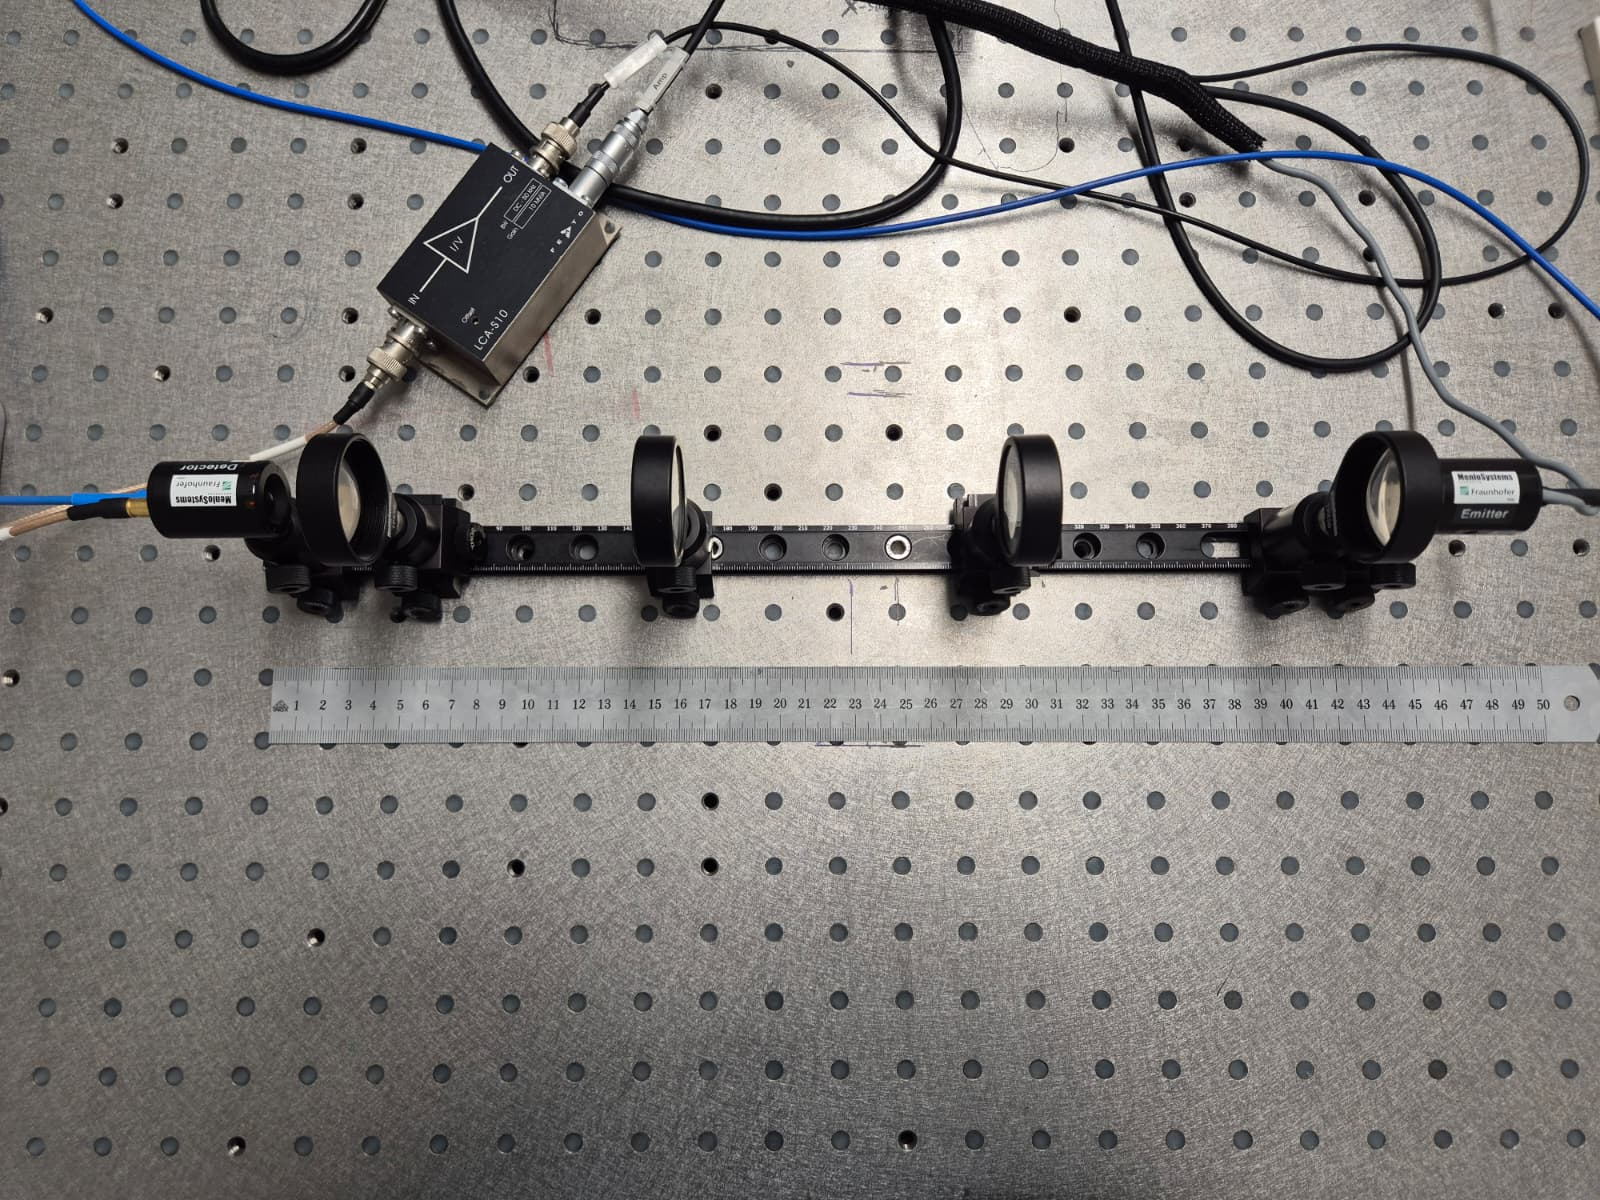
\includegraphics[height=3.4cm]{full_beam_path_aligned_top_view.jpeg}\hfill
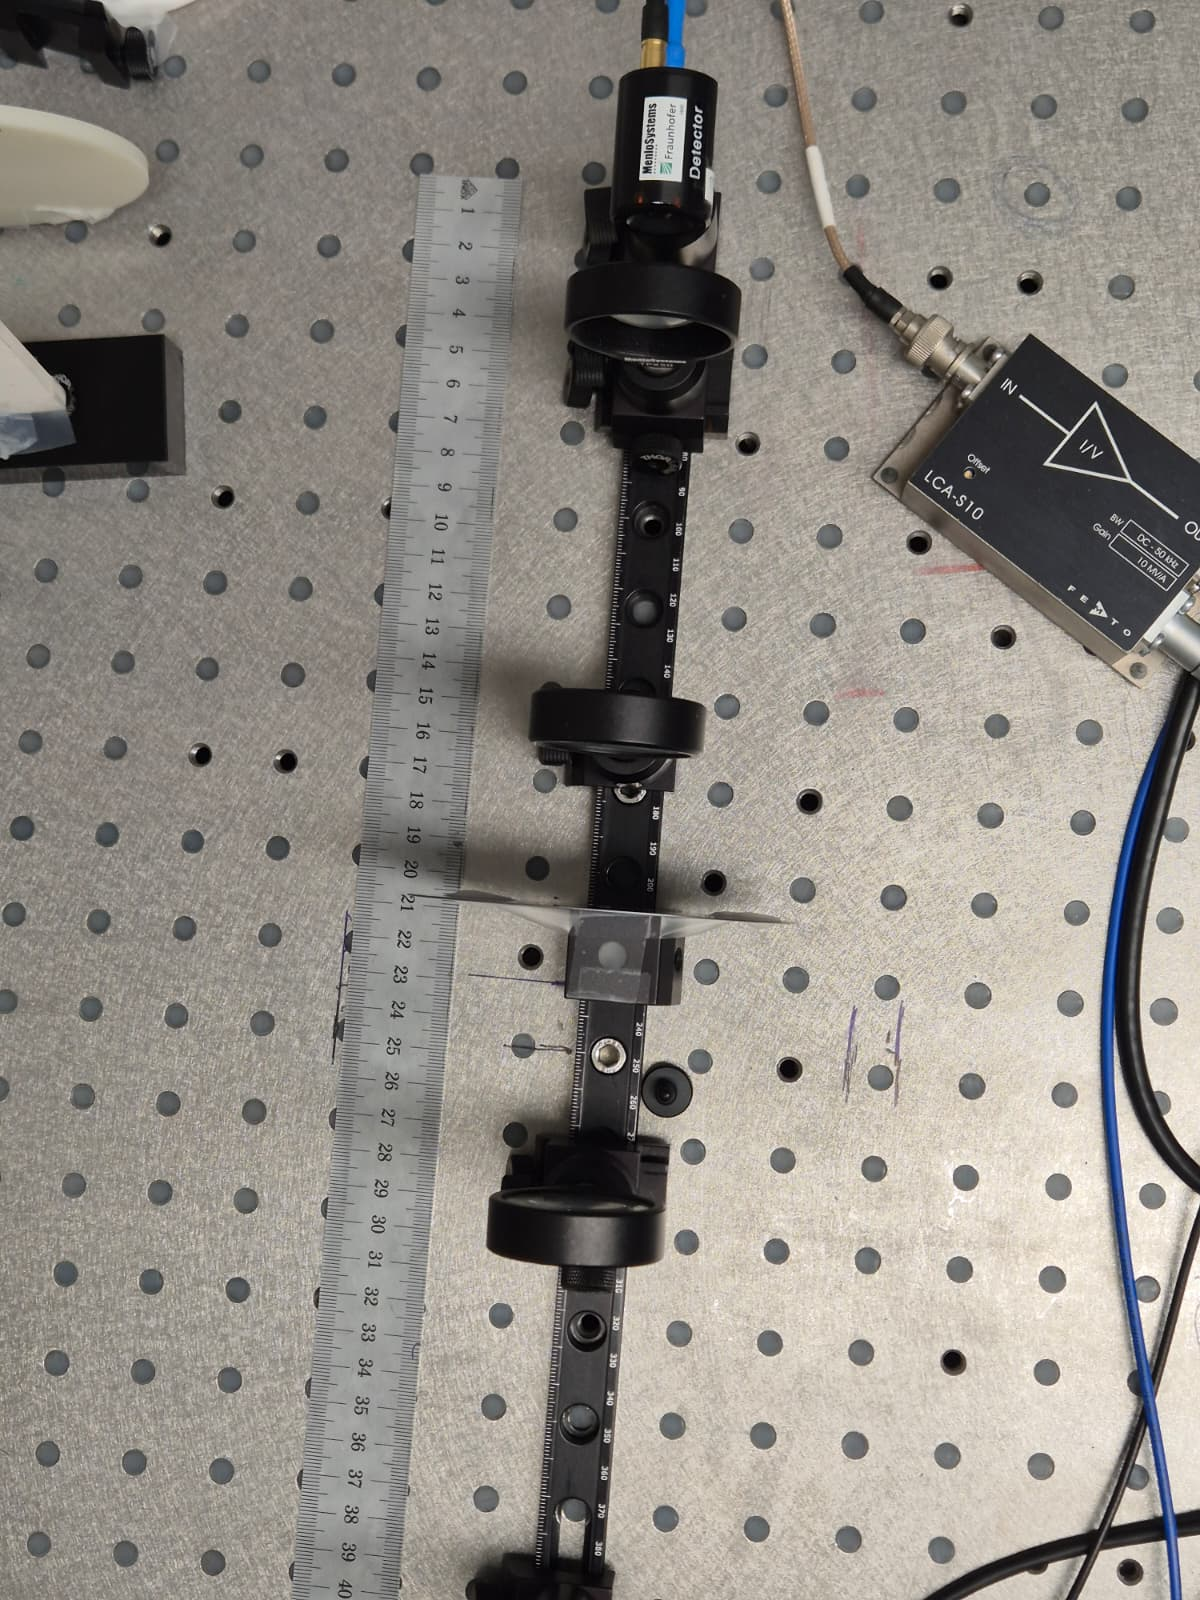
\includegraphics[height=3.4cm]{alignment_rail_top_sample_at_pinhole.jpeg}
\caption{Left: aligned THz path with emitter PCA (right side), detector PCA (left side) and the four TPX50 lenses; the transimpedance amplifier (Femto LCA-S10) is behind the rail. Right: a sample at the intermediate focus between lenses 2 and 3.}
\label{fig:setup}
\end{figure}

\section{Averaging and dynamic range}
After aligning each carrier and maximizing the detector current, the received pulse has a peak amplitude of 2.89 (arbitrary units) at $t = 43.9$\,ps on the shifted time axis (the raw scan starts at $-327$\,ps; all times below are quoted relative to that start). Fig.~\ref{fig:a1time} shows the four averaged traces and Table~\ref{tab:a1} the noise figures.

\begin{figure*}[!t]
\centering
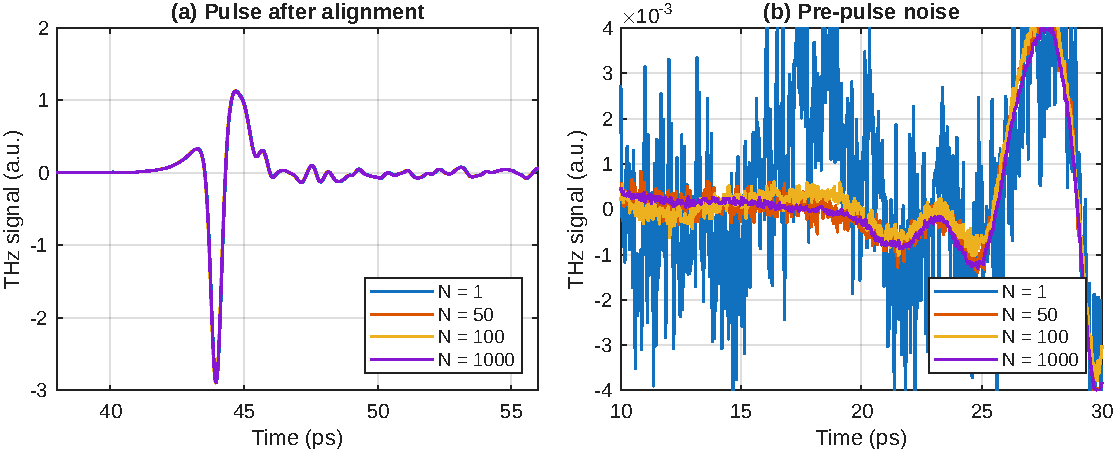
\includegraphics[width=0.85\textwidth]{fig_a1_time.pdf}
\caption{(a) Received pulse for $N$ = 1, 50, 100 and 1000 waveform averages; the four traces overlap because the alignment was not changed between scans. (b) Pre-pulse region. Averaging removes the white noise visible on the $N=1$ trace, but a coherent baseline structure (the slow oscillation and the bump near 27\,ps) is identical in all four traces and does not average down.}
\label{fig:a1time}
\end{figure*}

\begin{figure*}[!t]
\centering
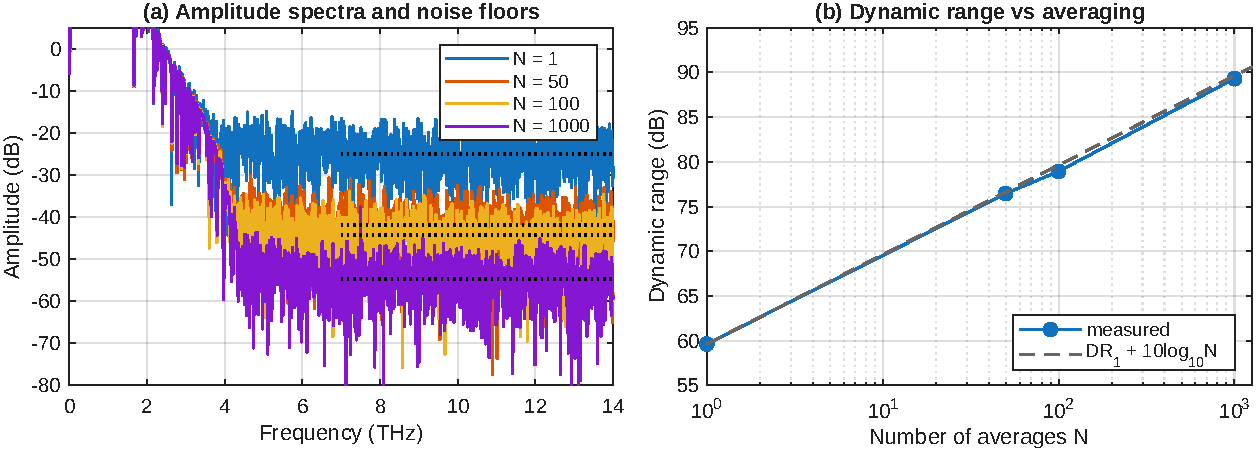
\includegraphics[width=0.85\textwidth]{fig_a1_spectra.pdf}
\caption{(a) Amplitude spectra of the four traces (4096-point FFT, Tukey window with $\alpha=0.1$). Dotted lines mark the noise floors, evaluated as the median level between 8 and 14\,THz. The sharp dips between 0.5 and 3\,THz are water vapour absorption lines. (b) Dynamic range against the number of averages, compared with $\mathrm{DR}_1 + 10\log_{10}N$.}
\label{fig:a1spec}
\end{figure*}

\begin{table}[!t]
\centering
\caption{Averaging study. $\sigma_t$ is the pre-pulse standard deviation (8--25\,ps), the floor is the median spectral level in 8--14\,THz, and DR is the peak spectral amplitude minus the floor.}
\label{tab:a1}
\setlength{\tabcolsep}{4pt}\begin{tabular}{rccccc}
\toprule
$N$ & $\sigma_t$ (a.u.) & floor (dB) & DR (dB) & $\Delta$DR (dB) & $10\log_{10}N$ \\
\midrule
   1 & $1.88\times10^{-3}$ & $-24.9$ & 59.6 &  0.0 &  0.0 \\
  50 & $4.57\times10^{-4}$ & $-41.8$ & 76.5 & 16.9 & 17.0 \\
 100 & $3.65\times10^{-4}$ & $-44.3$ & 78.9 & 19.3 & 20.0 \\
1000 & $4.43\times10^{-4}$ & $-54.6$ & 89.3 & 29.7 & 30.0 \\
\bottomrule
\end{tabular}
\end{table}

The spectral dynamic range DR, defined as the peak spectral amplitude minus the noise floor, grows by 16.9, 19.3 and 29.7\,dB for $N$ = 50, 100 and 1000; coherent averaging of white noise predicts $10\log_{10}N$ = 17.0, 20.0 and 30.0\,dB (Fig.~\ref{fig:a1spec}b). The white-noise model holds to within 0.7\,dB.

The time-domain noise behaves differently. The pre-pulse standard deviation drops from $1.9\times10^{-3}$ ($N=1$) to $3.6\times10^{-4}$ ($N=100$) and then stops improving ($N=1000$: $4.4\times10^{-4}$). Fig.~\ref{fig:a1time}(b) shows why: a coherent baseline structure repeats in every trace, so it survives averaging. Only the high-frequency part of the noise, which sets the spectral floor above 4\,THz, keeps falling with $N$. In practice the averaging buys usable bandwidth: the signal spectrum meets the $N=1$ floor near 3.5\,THz and the $N=1000$ floor near 4.2\,THz.

Two implementation notes. First, ScanControl saved the $N=1$ and $N=1000$ traces without the Tukey window it applied to the others (and saved no FFT files for them); the window was applied in post-processing before comparing spectra, and the two missing FFT exports were regenerated. Second, the FFT pipeline used here reproduces the ScanControl FFT files for $N=50$ and $N=100$ with an rms deviation of 0.12\,dB between 0.1 and 2\,THz (Fig.~\ref{fig:val}), which validates the rest of the processing chain.

\begin{figure*}[!t]
\centering
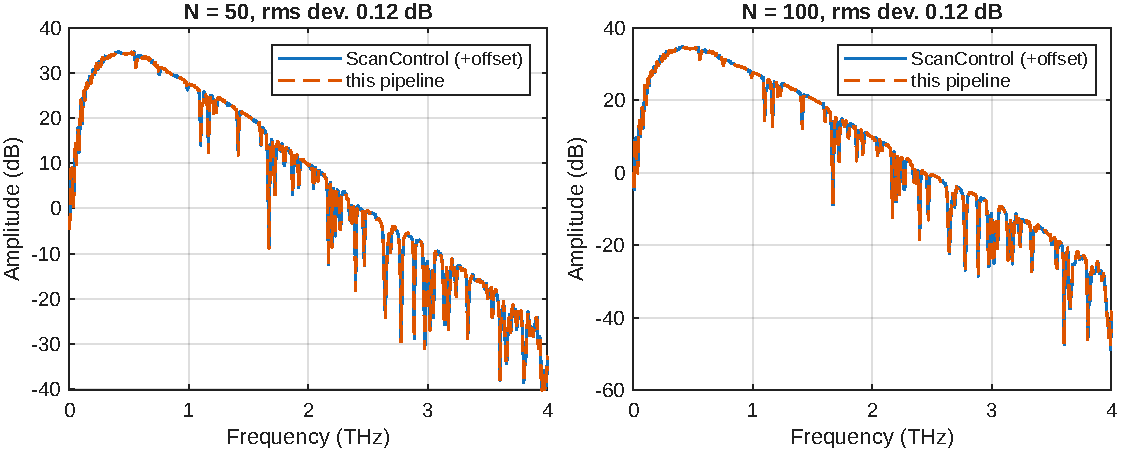
\includegraphics[width=0.85\textwidth]{fig_fft_validation.pdf}
\caption{FFT pipeline used here against the ScanControl FFT exports for $N=50$ and $N=100$, after removing a constant 34.7\,dB scale offset. The rms deviation is 0.12\,dB between 0.1 and 2\,THz.}
\label{fig:val}
\end{figure*}

\section{Permittivity and loss extraction}
\label{sec:method}
Each slab measurement is differential: a reference scan $E_{\mathrm{ref}}(t)$ without sample and a sample scan $E_{\mathrm{sam}}(t)$ with the slab at the intermediate focus \cite{proc}. The $N=100$ trace from Assignment~1 serves as the reference; it was recorded minutes before the slab series with the same averaging and the same window, unlike the $N=1000$ trace.

\subsection{Permittivity from the time delay}
The slab replaces a thickness $d$ of air with material of index $n = \sqrt{\varepsilon_r}$, so the pulse arrives later by $\tau_{\mathrm{dif}} = (n-1)\,d/c_0$. Inverting,
\begin{equation}
\varepsilon_r = \left(\frac{c_0(\tau_{\mathrm{dif}} + \tau_0)}{d}\right)^{\!2},
\qquad \tau_0 = d/c_0 .
\label{eq:eps}
\end{equation}
The arrival times are the minima of the dominant (negative) lobe, refined by parabolic interpolation; the scan step is 33.3\,fs, so $\tau_{\mathrm{dif}}$ contributes far less uncertainty than the thickness does. $\varepsilon_r$ is treated as constant over the band, per the course instructions \cite{proc}.

\subsection{Loss tangent from the transfer function}
The measured transfer function is $H(f) = E_{\mathrm{sam}}(f)/E_{\mathrm{ref}}(f)$. The slab is modelled as a transmission-line section of impedance $Z_s = Z_0\,(1 + j\tan\delta/2)/\sqrt{\varepsilon_r}$ and propagation constant $k_{zs} = \beta - j\alpha$, with $\beta = \omega\sqrt{\varepsilon_r}/c_0$ and $\alpha = \beta\tan\delta/2$, between two air lines \cite{proc}. The boundary conditions at the two interfaces give
\begin{equation}
\frac{V^+_{\mathrm{in}}}{V^+_{\mathrm{out}}}
= e^{jk_{zs}d}\,e^{-jk_{z0}d}\,
  \frac{1 + \Gamma_B e^{-2jk_{zs}d}}{(1+\Gamma_B)(1+\Gamma_A)},
\label{eq:tl}
\end{equation}
with $\Gamma_B = (Z_0 - Z_s)/(Z_0 + Z_s)$ and $\Gamma_A$ the input reflection coefficient of the loaded section. At each frequency, $\tan\delta(f)$ is the value for which $|H_{\mathrm{model}}|$ equals $|H_{\mathrm{meas}}|$, found by a grid search (a bracketing minimizer stalls on thick lossy slabs, where $|H_{\mathrm{model}}|$ is flat at zero over most of the $\tan\delta$ range). The attenuation per wavelength in the dielectric follows directly: $\alpha\lambda_d = \pi\tan\delta$ in nepers, or $27.3\tan\delta$ in dB.

Equation~\eqref{eq:tl} includes the Fabry--P\'erot etalon of the slab faces. That is only correct if the internal echo, which arrives $2nd/c_0$ after the main pulse, falls inside the 100\,ps scan window. For slab~1 (65\,ps round trip) and slab~3 (89\,ps) it does not, so for those two the model is reduced to the first transit only (Fresnel transmission at both faces plus propagation loss). The fit band is chosen per slab as the contiguous range where both spectra stay 15\,dB above their noise floors, typically 0.15 to 3\,THz, and 0.15 to 1.6\,THz for the lossy slab~3.

Where the etalon ripple is strong (the silicon wafers, interface reflection coefficient $\Gamma \approx 0.55$), the ripple period provides an independent permittivity estimate: sweeping $\varepsilon_r$ for the best ripple match gives 11.98 (slab~4) and 11.71 (slab~5), within 2.2\% of the delay values. For the low-contrast polymer slabs the ripple is weaker than the measurement noise and this cross-check is not meaningful, so the delay value is used throughout.

\section{Slab characterization}
Fig.~\ref{fig:a2time} shows the reference and the six slab traces, Table~\ref{tab:slabs} the extracted parameters, Fig.~\ref{fig:hfits} the transfer-function fits and Fig.~\ref{fig:tand} the frequency-resolved loss tangent. Four identifications are immediate: slab~3 matches the ceramic ($\varepsilon_r$ within 1.5\% of the tabulated 7.55), slabs~4 and 5 match silicon (within 2.1\% of 11.90), and slab~6 matches Teflon (within 2.2\% of 2.10). Slab~2, once its thickness is settled (Sec.~\ref{sec:slab2}), matches Gore-Tex within 3.1\%. Slab~1 is the outlier and is discussed in Sec.~\ref{sec:slab1}.

\begin{figure*}[!t]
\centering
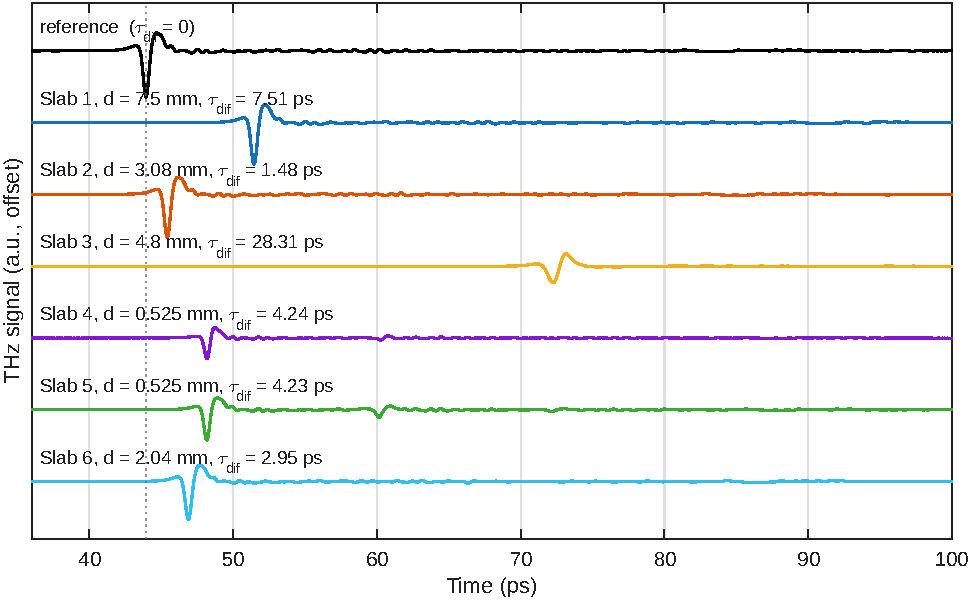
\includegraphics[width=0.8\textwidth]{fig_a2_time.pdf}
\caption{Reference pulse and the six slab measurements (offset vertically). The dotted line marks the reference arrival time. The echo of the slab~5 etalon is visible 12\,ps after its main pulse, near 60\,ps.}
\label{fig:a2time}
\end{figure*}

\begin{table}[!t]
\centering
\caption{Extraction summary. $\varepsilon_r$ from \eqref{eq:eps}; $\tan\delta$ from the $|H|$ fit at 0.5\,/\,1.0\,THz; attenuation per wavelength at 0.5\,THz. The last column is the deviation of $\varepsilon_r$ from the closest entry of the lab-manual table.}
\label{tab:slabs}
\setlength{\tabcolsep}{3pt}\begin{tabular}{lcccccll}
\toprule
 & $d$ & $\tau_{\mathrm{dif}}$ & $\varepsilon_r$ & $\tan\delta$ & dB/$\lambda$ & material & dev. \\
 & (mm) & (ps) &  & (0.5/1\,THz) &  &  & (\%) \\
\midrule
Slab 1 & 7.5   &  7.51 &  1.69 & 0.0006/0.0010 & 0.02 & Gore-Tex$^{\ast}$ & $+25.2$ \\
Slab 2 & 3.08  &  1.48 &  1.31 & 0.0019/0.0026 & 0.05 & Gore-Tex & $-3.1$ \\
Slab 3 & 4.8   & 28.31 &  7.66 & 0.0056/0.0131 & 0.15 & Ceramic  & $+1.5$ \\
Slab 4 & 0.525 &  4.24 & 11.72 & 0.0531/0.0138 & 1.45 & Silicon  & $-1.5$ \\
Slab 5 & 0.525 &  4.23 & 11.66 & 0.0075/0.0028 & 0.20 & Silicon  & $-2.1$ \\
Slab 6 & 2.04  &  2.95 &  2.05 & 0.0048/0.0082 & 0.13 & Teflon   & $-2.2$ \\
\bottomrule
\end{tabular}
\par\smallskip
\footnotesize $^{\ast}$Nearest table entry; see Sec.~\ref{sec:slab1}.
\end{table}

\begin{figure*}[!t]
\centering
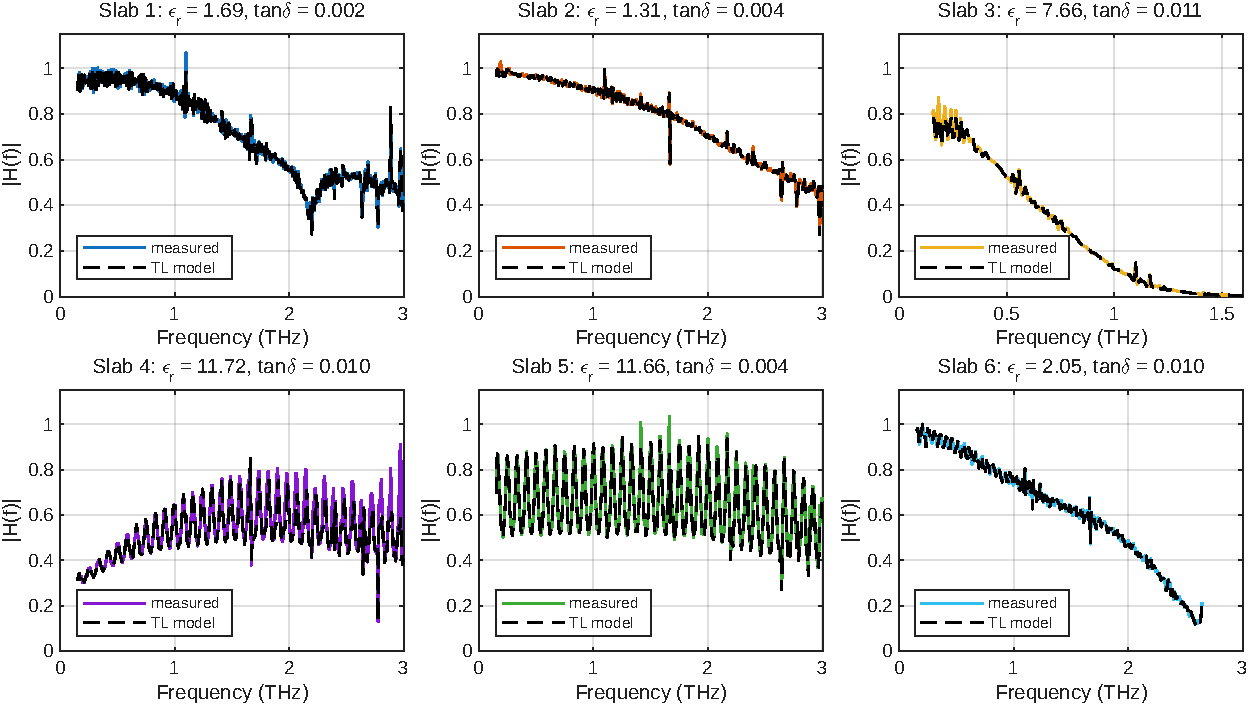
\includegraphics[width=0.92\textwidth]{fig_a2_Hfits.pdf}
\caption{Measured $|H(f)|$ (colour) and fitted transmission-line model (dashed) for the six slabs. The silicon wafers show the etalon ripple with period $c_0/(2nd) \approx 83$\,GHz; the model reproduces both period and amplitude. Slabs 1 and 3 use the single-transit model because their internal echo falls outside the scan window. The isolated spikes (e.g.\ near 1.1 and 1.65\,THz) are division artifacts at water vapour lines.}
\label{fig:hfits}
\end{figure*}

\begin{figure*}[!t]
\centering
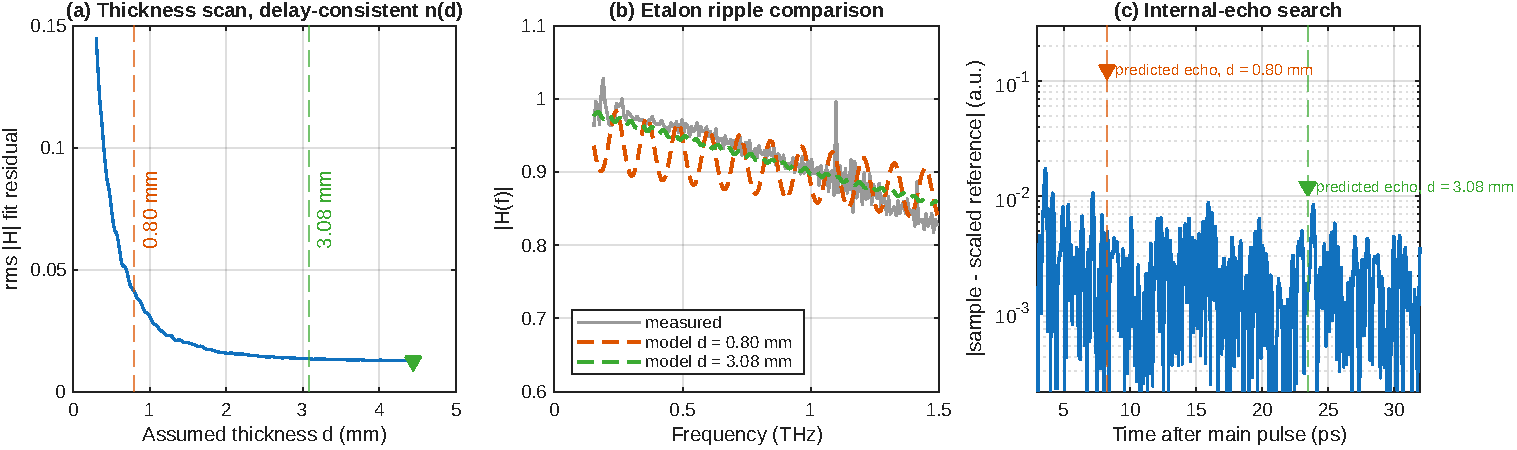
\includegraphics[width=0.92\textwidth]{fig_slab2_dscan.pdf}
\caption{Settling the slab~2 thickness. (a) Fit residual against assumed thickness, with $n(d)$ constrained by the measured delay; 0.8\,mm is clearly worse, while everything above $\approx 3$\,mm fits equally well. (b) The 0.8\,mm candidate requires an etalon ripple of about $\pm 10$\% with a 120\,GHz period; the measurement is smooth. (c) Residual after subtracting the shifted, scaled reference: a 0.8\,mm slab would put a 0.13\,a.u.\ echo at $+8.3$\,ps, an order of magnitude above what is observed.}
\label{fig:dscan}
\end{figure*}

\begin{figure}[!t]
\centering
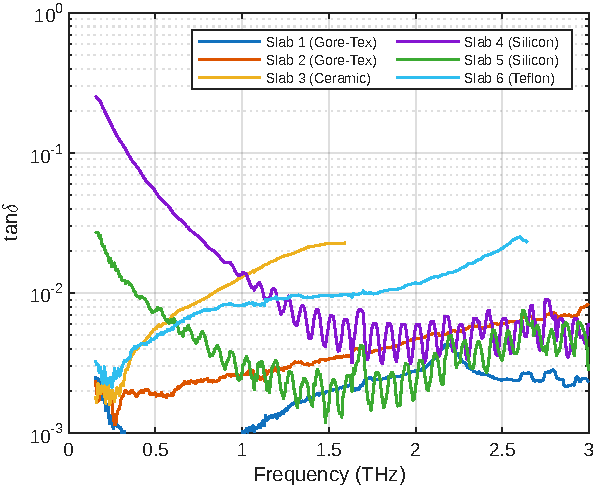
\includegraphics[width=\columnwidth]{fig_a2_tand_col.pdf}
\caption{Extracted $\tan\delta(f)$, smoothed over 9 frequency bins. The silicon wafers fall off roughly as $1/f$, as expected for free-carrier conduction loss with constant conductivity; the polymers and the ceramic rise with frequency. The residual oscillation on the silicon curves is the imperfectly cancelled etalon ripple.}
\label{fig:tand}
\end{figure}

\begin{figure}[!t]
\centering
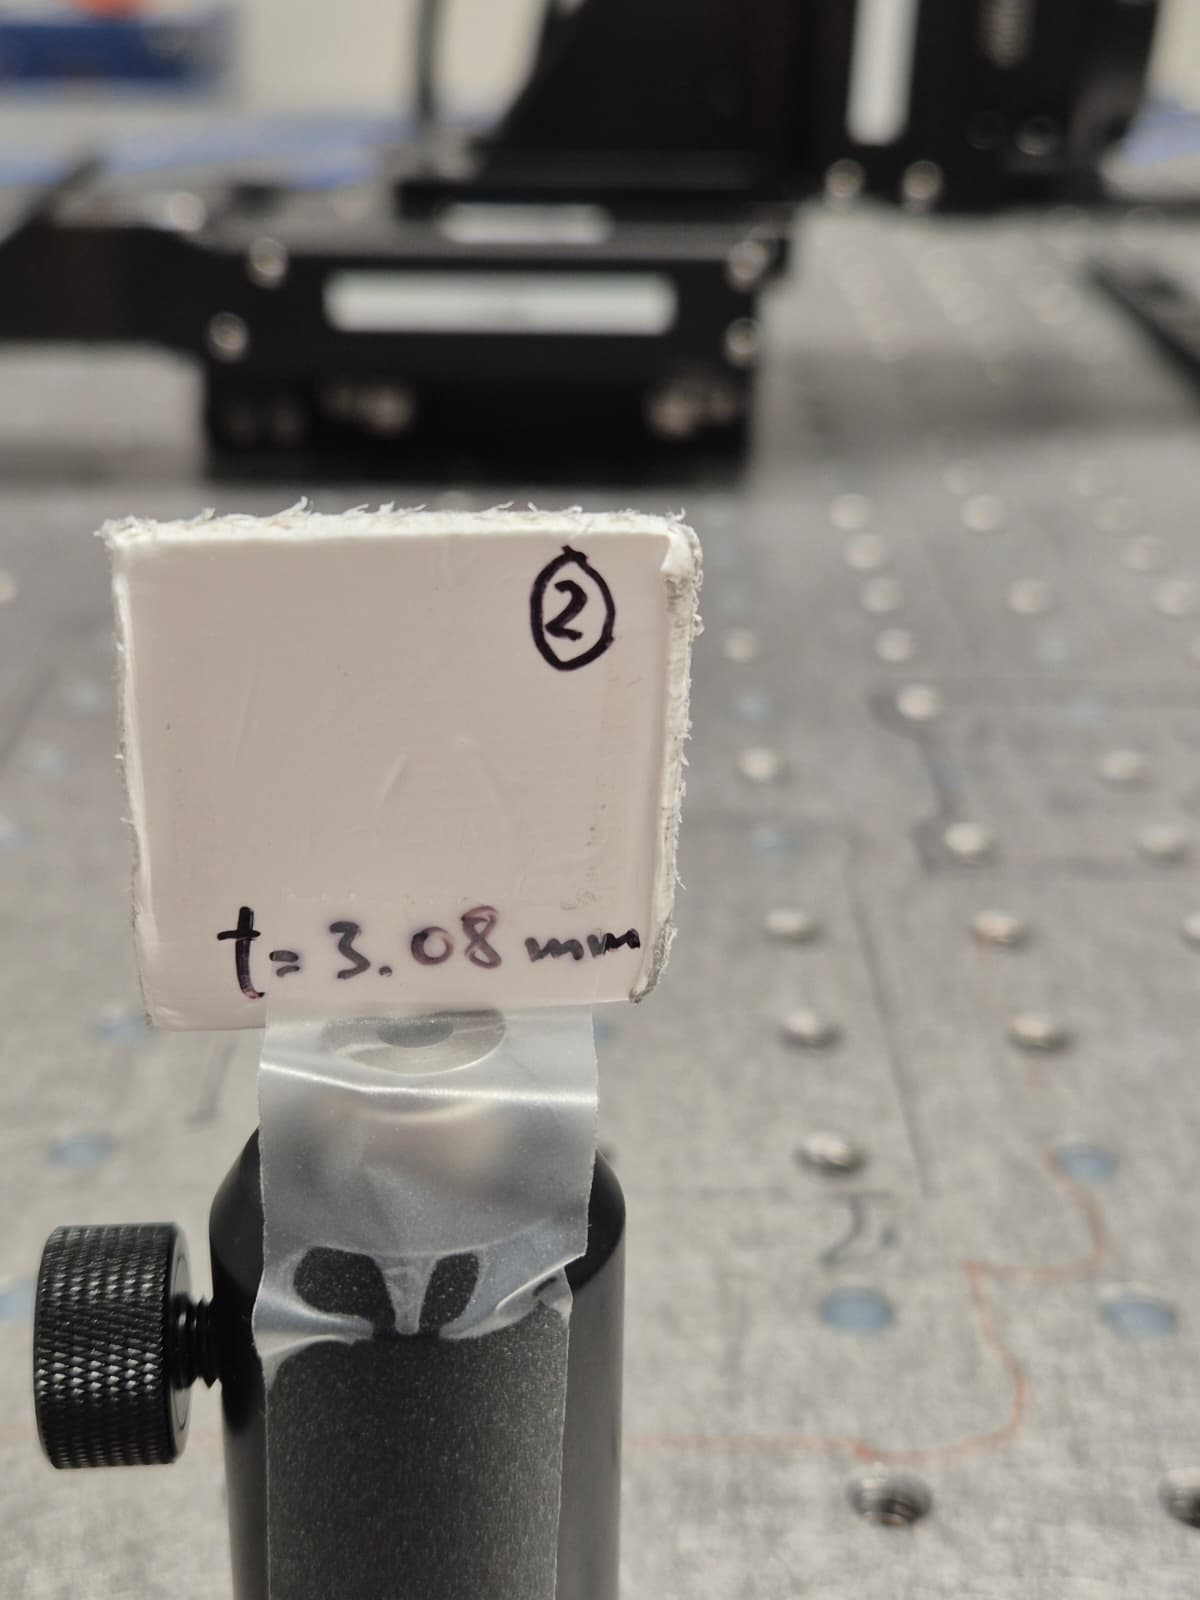
\includegraphics[height=3.6cm]{slab2_label_t3.08mm_holder.jpeg}\hspace{0.8em}
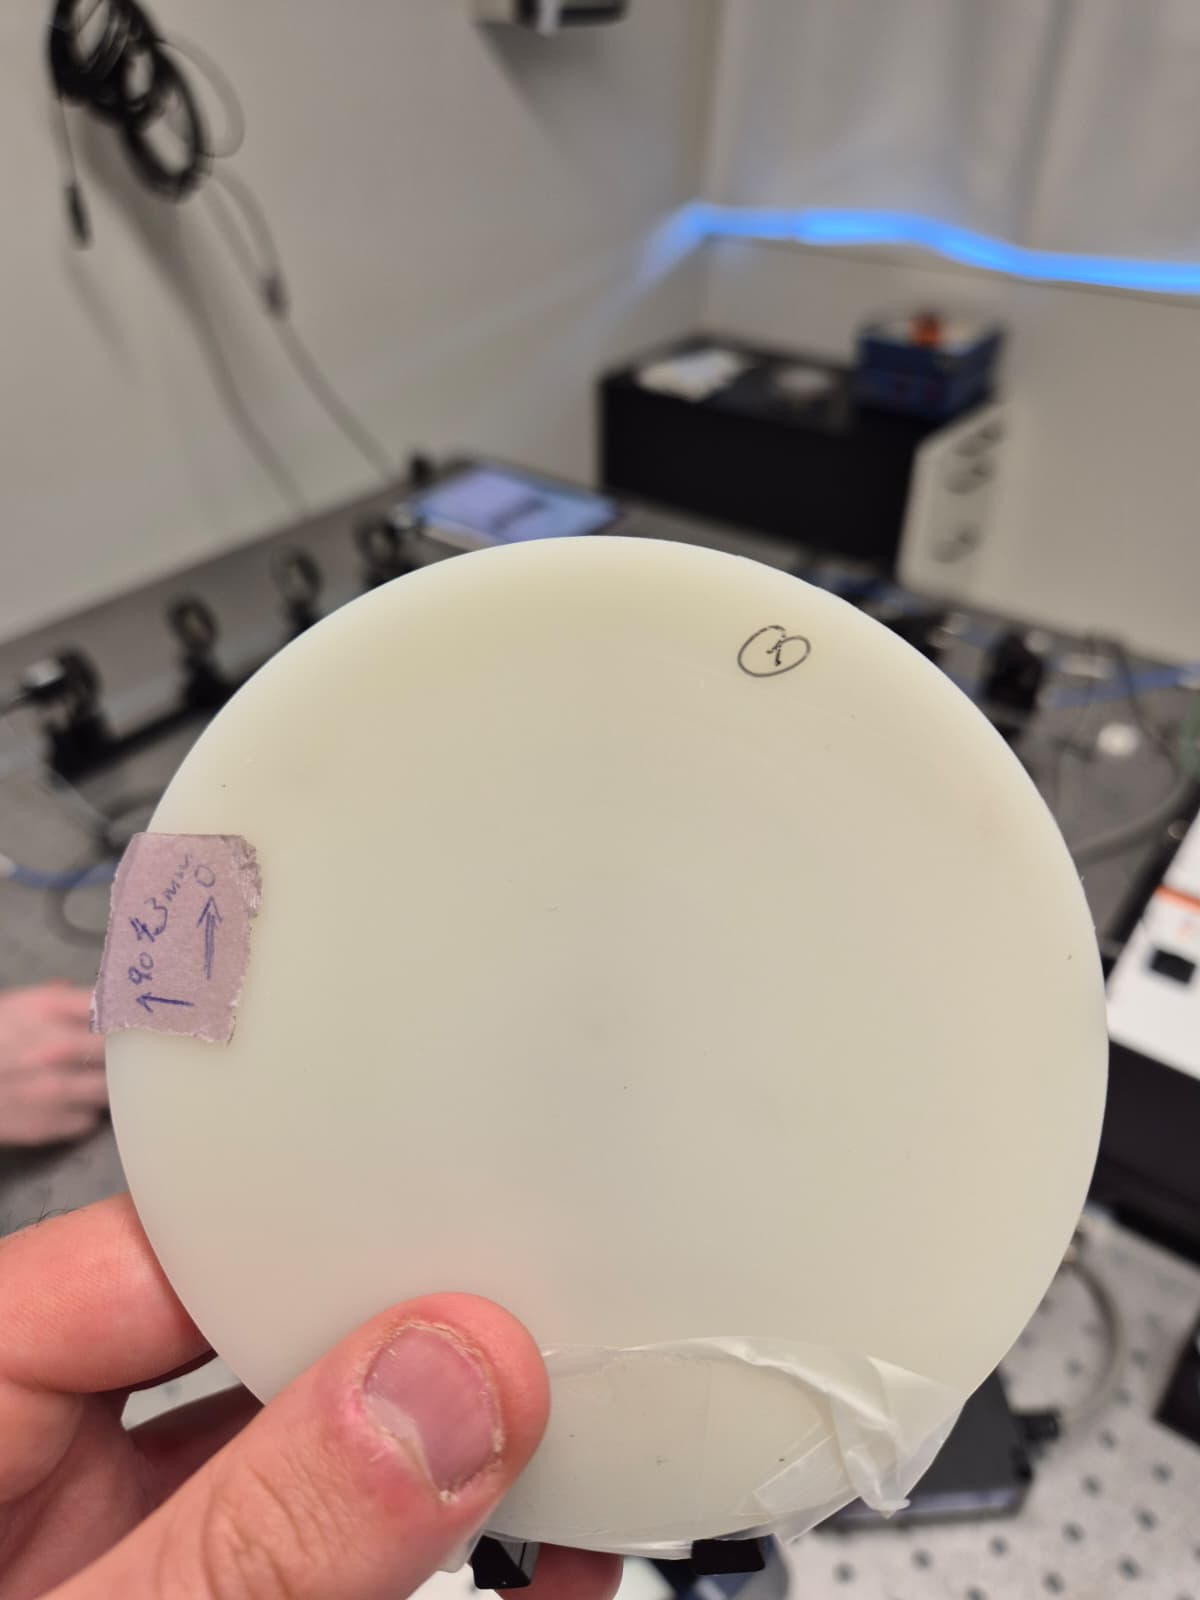
\includegraphics[height=3.6cm]{slab1_round_white_orientation_arrows.jpeg}
\caption{Left: slab~2 in its holder, marked $t=3.08$\,mm. The frayed, fibrous edges are typical of expanded PTFE (Gore-Tex), which matches the extracted $\varepsilon_r = 1.31$. Right: slab~1, a 7.5\,mm disc with orientation arrows.}
\label{fig:photos}
\end{figure}

\subsection{Silicon wafers and resistivity}
The two wafers have the same permittivity ($n$ = 3.423 and 3.414, within 0.3\% of the 3.418 reported for high-resistivity silicon in \cite{grisch}) but very different loss. For conduction loss, $\tan\delta = \sigma/(\omega\varepsilon_0\varepsilon_r)$, so a constant conductivity appears as $\tan\delta \propto 1/f$, which is what Fig.~\ref{fig:tand} shows below 1.5\,THz. The median equivalent conductivity gives $\rho = 37$\,$\Omega\cdot$cm for slab~5, in fair agreement with the 33\,$\Omega\cdot$cm printed on that wafer, and $\rho = 9$\,$\Omega\cdot$cm for slab~4, the lossier and presumably more doped of the two. This agreement is a useful end-to-end check of the loss extraction, since the wafer label comes from an independent four-point-probe measurement.

\subsection{Resolving the slab 2 thickness}
\label{sec:slab2}
The data file for slab~2 is named \texttt{Slab2\_0.8}, but the sample itself is marked $t = 3.08$\,mm (Fig.~\ref{fig:photos}). The measured delay alone cannot distinguish the two: with $d=0.8$\,mm it gives $\varepsilon_r = 2.44$ (HDPE-like), with $d=3.08$\,mm it gives $\varepsilon_r = 1.31$ (Gore-Tex-like). The etalon, however, fixes the optical thickness independently. Fig.~\ref{fig:dscan} shows three tests, all of which reject 0.8\,mm: the rms $|H|$ fit residual is 0.041 for 0.8\,mm against 0.014 for 3.08\,mm; the 120\,GHz ripple that a 0.8\,mm slab of $\varepsilon_r=2.44$ must produce is absent from the measured $|H|$; and the internal echo that should appear 8.3\,ps after the main pulse with amplitude $\Gamma^2 \cdot 2.68 \approx 0.13$\,a.u.\ is not there (the residual at that delay stays below 0.011\,a.u.). Near $+23.5$\,ps, where the 3.08\,mm echo belongs, the residual reaches 0.008\,a.u., consistent with the 0.012\,a.u.\ predicted for the much weaker $\Gamma = 0.067$ of a low-index slab. All results in this report therefore use $d = 3.08$\,mm; the file name records the thickness of a different sample or a typo.

\subsection{Slab 1}
\label{sec:slab1}
Slab~1 gives $\varepsilon_r = 1.69$, between Gore-Tex (1.35) and Teflon (2.10) and 25\% from the nearest table entry. The extraction itself is not suspect: the delay of 7.51\,ps over 7.5\,mm is the largest of the polymer slabs and the least sensitive to timing error, and the single-transit $|H|$ model fits with $\tan\delta \approx 10^{-3}$, the lowest loss of all six samples. A plausible reading is a porous PTFE of intermediate density: expanded PTFE spans a permittivity range between roughly 1.2 and the bulk 2.1 depending on air fraction, and the table's 1.35 represents one specific density. The orientation arrows on the disc (Fig.~\ref{fig:photos}, right) suggest an engineered, possibly anisotropic material, and a measurement at the orthogonal polarization would test that. Within the supplied table the closest entry is Gore-Tex, and the very low loss at least excludes the denser candidates.

\section{Conclusion}
The aligned spectrometer delivers a 89.3\,dB spectral dynamic range at $N=1000$ averages, and the measured improvement with averaging follows $10\log_{10}N$ to within 0.7\,dB; the time-domain baseline, in contrast, is limited by coherent structure at the $4\times10^{-4}$ level that averaging does not remove. The delay-plus-transmission-line extraction identified five of the six slabs within 3.1\% of the reference permittivities (silicon $\times 2$, ceramic, Teflon, Gore-Tex), reproduced the labelled resistivity of the 33\,$\Omega\cdot$cm silicon wafer to within 12\%, and settled the slab~2 thickness conflict in favour of the 3.08\,mm marking using the etalon ripple and the missing internal echo. Slab~1 ($\varepsilon_r = 1.69$, $\tan\delta \approx 10^{-3}$) does not match any table entry within 25\% and is most consistent with a porous PTFE of intermediate density.

\begin{thebibliography}{9}
\bibitem{labman} M. Alonso-delPino, ``EE4730 Time Domain Laboratory,'' TU Delft, 2026.
\bibitem{proc} M. Alonso-delPino, ``Project: Material characterization using a time domain system,'' EE4730 processing notes, TU Delft, 2026.
\bibitem{jepsen} P. U. Jepsen, D. G. Cooke, and M. Koch, ``Terahertz spectroscopy and imaging -- modern techniques and applications,'' \emph{Laser Photon.\ Rev.}, vol.~5, no.~1, pp.~124--166, 2011.
\bibitem{grisch} D. Grischkowsky, S. Keiding, M. van Exter, and Ch. Fattinger, ``Far-infrared time-domain spectroscopy with terahertz beams of dielectrics and semiconductors,'' \emph{J. Opt.\ Soc.\ Am.\ B}, vol.~7, no.~10, pp.~2006--2015, 1990.
\end{thebibliography}

\end{document}
